\section{定积分的定义与性质}
\label{sec:ru-riemann-integral}

\subsection{黎曼和}
\label{sec:ru-riemann-sums}

速度恒为$v$时，时长$\Delta t$内的位移是$v\,\Delta t$。速度随时间变化时，可以把时间区间切成许多小段，每段内速度变化不大，就用该段某一时刻的速度乘以段长近似这一段的位移，再把各段加起来。
同样的做法用于曲线下的面积：把底边切成小段，每段用一个矩形近似。下面把这个过程写成一般的定义。

设$f$定义在$[a,b]$上。取有限个分点$a=x_0<x_1<\cdots<x_n=b$，称为$[a,b]$的一个\term{分割}（partition）$P$，记$\Delta x_i=x_i-x_{i-1}$，并称最长小段的长度$\|P\|=\max_i\Delta x_i$为分割的网格尺度。
在每段中任取一点$\xi_i\in[x_{i-1},x_i]$，称和
\[
 S(f,P,\xi)=\sum_{i=1}^nf(\xi_i)\,\Delta x_i
\]
为一个\term{黎曼和}（Riemann sum）。$f\geq0$时每一项是一个矩形的面积；$f$取负值时，横轴下方的矩形按负号计入，所以黎曼和是带符号的累计。
黎曼和依赖两种选择：分割$P$与取样点$\xi$。让$\|P\|\to0$是要求每一段都变短，而不只是增加分点的个数。

\begin{definition}[黎曼积分]
\label{def:ru-riemann-integral}
设$f:[a,b]\to\mathbb R$有界。若存在实数$A$，使对每个$\varepsilon>0$都存在$\delta>0$，只要$\|P\|<\delta$，无论怎样选取样点都有$|S(f,P,\xi)-A|<\varepsilon$，
就称$f$在$[a,b]$上\term{黎曼可积}（Riemann integrable），称$A$为它的定积分，记作$\int_a^bf(x)\,\mathrm dx$。
\end{definition}
定义同时控制了全部足够细的分割与全部取样方式。只检查某一列等距分割配某种取样点是不够的：在$[0,1]$上，有理点取$1$、无理点取$0$的指示函数$\mathbb I_{\mathbb Q}$，
若总取等距分割的中点（中点都是有理数），黎曼和恒为$1$；若取样点全选无理数，黎曼和恒为$0$。两种取样都能任意细，却给出不同的结果，所以这个函数不黎曼可积。
积分变量只在积分号内部使用，换名不改变结果：$\int_a^bf(x)\,\mathrm dx=\int_a^bf(t)\,\mathrm dt$。

定积分是带符号的累计，不同于几何面积。$\int_0^{2\pi}\sin x\,\mathrm dx=0$，因为横轴上下两部分相互抵消；而正弦曲线与横轴围成的几何面积是$\int_0^{2\pi}|\sin x|\,\mathrm dx=4$。
图~\ref{fig:ru-riemann-sums}(a)画出了一个取样点不规则、分割不等距的黎曼和，负值部分以红色计入。

\begin{figure*}[!htbp]
 \centering
 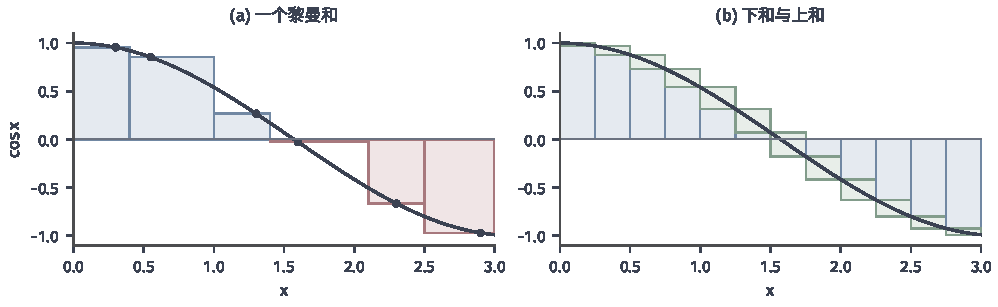
\includegraphics[width=169mm]{figures/01-mathematical-preliminaries-upper/02-real-numbers-and-univariate-functions/matplotlib/riemann-sums/figure.pdf}
 \caption{$f(x)=\cos x$在$[0,3]$上的累计。(a)不等距分割（$6$段）的一个黎曼和，黑点为各段的取样点，蓝色矩形按正号计入，红色矩形按负号计入。(b)同一函数在$12$段等距分割上的下和与上和：蓝色为下和，加上绿色部分得到上和，绿色总面积就是$U-L$。分割加细时这一差值趋于零，函数可积。图为解析示例。}
 \label{fig:ru-riemann-sums}
\end{figure*}

\subsection{可积性}
\label{sec:ru-integrability}

直接检查所有分割和取样并不方便。把每一段上可能的取样值夹在上下确界之间，就能用两个与取样无关的和控制全部黎曼和。
设$f$在$[a,b]$上有界，对分割$P$，记$m_i,M_i$为$f$在$[x_{i-1},x_i]$上的下确界与上确界，定义下和与上和
\[
 L(f,P)=\sum_im_i\,\Delta x_i,\qquad U(f,P)=\sum_iM_i\,\Delta x_i.
\]
同一分割下的任意黎曼和都满足$L(f,P)\leq S(f,P,\xi)\leq U(f,P)$。这里用确界而不用最值，因为有界函数在小段上未必取到最值。

加入新的分点时，一段被拆成几段，每个子段上的下确界不小于原段的下确界，上确界不大于原段的上确界，所以下和不减、上和不增。
任意两个分割有公共加细，因此任意下和都不超过任意上和。于是下积分$\sup_PL(f,P)$不超过上积分$\inf_PU(f,P)$。
\begin{theorem}[Darboux判据]
\label{thm:ru-darboux-criterion}
有界函数$f$在$[a,b]$上黎曼可积，当且仅当对每个$\varepsilon>0$，存在分割$P$使$U(f,P)-L(f,P)<\varepsilon$。此时积分等于上积分和下积分的共同值。
\end{theorem}
\begin{proof}
设条件成立。固定一个满足$U(f,P_0)-L(f,P_0)<\varepsilon$的分割$P_0$，设它有$k$个内分点，且$|f|\leq M$。对另一个分割$Q$，不含$P_0$分点的小段落在$P_0$的某一段内，沿用该段的上下界；
含有$P_0$分点的小段至多$k$个，总长度至多$k\|Q\|$，函数在其上的振幅至多为$2M$。所以$U(f,Q)-L(f,Q)\leq\varepsilon+2Mk\|Q\|$，$\|Q\|$足够小时小于$2\varepsilon$。
任意黎曼和与上下积分的共同值都夹在$L(f,Q)$与$U(f,Q)$之间，两者之差小于$2\varepsilon$，这正是黎曼可积的定义。
反过来，若$f$可积，取足够细的分割，在每段上分别取接近上确界与接近下确界的取样点，两组黎曼和都接近积分值，又分别接近$U$与$L$，所以$U-L$可以任意小。
\end{proof}
判据只用到实数的确界与有限分割，不需要事先知道积分值。图~\ref{fig:ru-riemann-sums}(b)中的绿色部分就是$U-L$。

由判据可以判定几类函数可积。闭区间上的连续函数一致连续，给定$\varepsilon>0$，取$\delta$使距离小于$\delta$的两点函数值相差小于$\varepsilon/(b-a)$；
网格尺度小于$\delta$时每段的振幅$M_i-m_i<\varepsilon/(b-a)$，所以$U-L<\varepsilon$。单调函数也可积：若$f$单调不减，取$n$等分，$M_i=f(x_i)$、$m_i=f(x_{i-1})$，求和相消得$U-L=(f(b)-f(a))(b-a)/n\to0$。
只有有限个间断点的有界函数同样可积：用总长度很小的有限个区间把间断点隔开，这部分对$U-L$的贡献不超过$2M$乘以总长度，其余部分按连续函数处理。

可积性有真实的限制。前面的$\mathbb I_{\mathbb Q}$在$[0,1]$的每个小区间上都同时取到$0$和$1$，所以对任意分割$L=0$、$U=1$，差值不随分割加细而减小，Darboux判据不成立。
困难不在于分割不够细，而在于函数在任意短的区间内都剧烈振荡。这类函数能否以另一种方式累计，是第~\ref{chap:measurable-functions}章的问题。

\subsection{积分的性质}
\label{sec:ru-integral-properties}

以下性质都从黎曼和直接得到。若$f,g$在$[a,b]$上可积，对同一分割和同一组取样点，$S(\alpha f+\beta g,P,\xi)=\alpha S(f,P,\xi)+\beta S(g,P,\xi)$，取极限便得线性
\[
 \int_a^b(\alpha f+\beta g)=\alpha\int_a^bf+\beta\int_a^bg.
\]
对$a<c<b$，把$c$作为分点，左右两段的黎曼和相加就是全区间的黎曼和，于是$\int_a^bf=\int_a^cf+\int_c^bf$。约定$\int_b^af=-\int_a^bf$、$\int_a^af=0$后，这个等式对$a,b,c$的任意顺序都成立。
若$f\leq g$，每个黎曼和都保持这一大小关系，所以$\int_a^bf\leq\int_a^bg$。$|f|$也可积，因为它在每段上的振幅不超过$f$的振幅；由$-|f|\leq f\leq|f|$得$\bigl|\int_a^bf\bigr|\leq\int_a^b|f|$。
乘积$fg$也可积，但积的积分一般不等于积分的积：在$[0,1]$上$\int x\cdot x\,\mathrm dx=1/3$，而$(\int x\,\mathrm dx)^2=1/4$。

保序性给出两个后面反复使用的估计。第一个是误差估计：若$|f-g|\leq\eta$在$[a,b]$上处处成立，则
\[
 \Bigl|\int_a^bf-\int_a^bg\Bigr|\leq\int_a^b|f-g|\leq\eta\,(b-a),
\]
函数的统一误差界乘以区间长度，就是积分的误差界。第~\ref{sec:ru-limit-interchange}节用它交换极限与积分，第~\ref{sec:ru-numerical-quadrature}节用它估计求积误差。
第二个是积分平均值：若$f$在$[a,b]$上连续，$m\leq f\leq M$分别为最小值与最大值，则$m\leq\frac1{b-a}\int_a^bf\leq M$，由介值定理，存在$c\in[a,b]$使
\[
 \int_a^bf(x)\,\mathrm dx=f(c)\,(b-a).
\]
$\frac1{b-a}\int_a^bf$称为$f$在$[a,b]$上的平均值，它是有限个函数值的算术平均在连续情形下的对应物。
